\documentclass[12pt]{article}
\usepackage[francais]{babel}
\usepackage[utf8]{inputenc}
\usepackage{graphicx}
\usepackage{amsmath}
\usepackage{amsfonts}
\usepackage{amssymb}




\addtolength{\hoffset}{-1cm}
\addtolength{\textwidth}{2cm} 
\addtolength{\voffset}{-1cm}
\addtolength{\textheight}{2cm} 

\begin{document}

\begin{titlepage}
\begin{center}

\hfill
\vfill
\bigskip
\huge{ 
\includegraphics[width=60,height=50]{logo.png} 

\includegraphics[width=80,height=50]{lh.png} \\
 Rapport de stage \\ M2 MATIS  \\ \\ \\ \\ \\
 } 
\vfill
\bigskip 
\Huge 
\bigskip 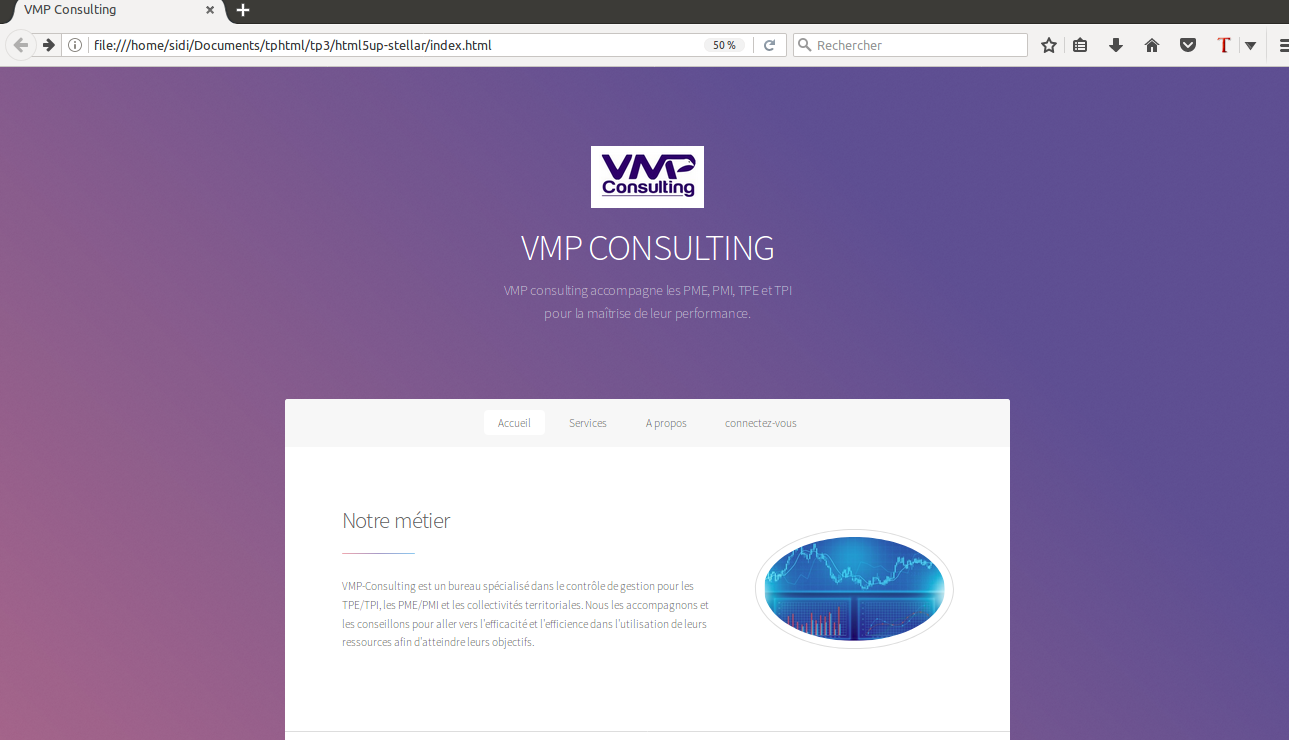
\includegraphics[width=120,height=150]{design1.png}} \\ \\
 Développement d'un portail web pour VMP Consulting \par 
\vfill

\Large \begin{flushleft}
 Réalisé par:\\ sidi Maouloud \par
\end{flushleft}
		 
		  \begin{flushright}
		                    sous la direction de:\\  M. ould Maouloud
		                   \end{flushright}



		 
\vfill
\Large Université du Havre \par \Large VMP Consulting		
		\bigskip 
\bigskip

\Large
28 Octobre 2017
\end{center}
\end{titlepage}

\section*{Remerciements}
Je tiens á transmettre ma gratitude et mon affection à ma mère, mon père  et ma
sœur, ainsi que mes proches pour leur patience et leur soutien.\\ \\

J’adresse mes remerciements à  M. sidi ould MAOULOUD, de m’avoir accueillie pour faire mon
stage au sein de son entreprise, ainsi pour son aide et  ses  remarques pertinentes.  \\ \\
J’aimerais aussi remercier M. Laurent Amanton  et tous mes enseignants de l’université du havre
qui m’ont accompagné 
au cours de cette année.\\ \\


\newpage

\section*{Résumé}
\textbf{VMP-CONSULTING}  est un bureau spécialisé dans le contrôle de gestion pour les TPE/TPI, les PME/PMI et les collectivités territoriales. Il les accompagne et les conseille pour aller vers l'efficacité et l'efficience dans l'utilisation de leurs ressources afin d'atteindre leurs objectifs.\\
Pour mieux servir ses clients, \textbf{VMP-CONSULTING}  veut avoir un portail web pour 
mettre en œuvre un espace de travail unique pour les clients, 
 proposer aux clients un accès privilégié et personnalisé à divers services en
ligne, et 
développer des outils qui permettent aux clients de réagir avec les contenus du
portail.\\
L'objectif de ce stage est de réaliser ce site web.


\section*{Abstract}
Whatever the activity, today all companies are confronted with increased competitive pressure, technological changes ... To enable managers and operational staff to devote themselves entirely to their core business, support in managing The company is a necessity not to say an obligation. In this area, not all businesses are housed in the same category, particularly small businesses and small businesses. The lack of management tools is mainly linked to a problem of means although sometimes it can be a problem of awareness of the utility and the benefit brought by these tools.\\
\textbf{VMP-CONSULTING}  is an office specializing in management control for small and medium-sized enterprises (SMEs), SMEs and local authorities. He accompanies them and advises them to move towards efficiency and efficiency in the use of their resources in order to achieve their objectives.\\
To better serve its customers, \textbf{VMP-CONSULTING}  wants to have a web portal for
implement a unique workspace for customers,
 offer customers privileged and personalized access to various services in
line, and
develop tools that enable clients to react with the contents of the
portal.\\
The objective of this traineeship is to realize this website

\newpage

\tableofcontents
\newpage



\section{Introduction et Problématique}

Un portail web est une plate-forme collaborative dont la fonction première est de proposer aux internautes des ressources et services numériques en rapport avec un thème, un domaine d’intérêt et dédié à chaque communauté particulière (les collaborateurs, les partenaires, les clients ou encore les fournisseurs …).\\
Il s’agit d’un espace de travail unique, personnalisé et sécurisé avec des droits d’accès par utilisateur.\\
L’enjeu pour une entreprise aujourd'hui est d’adresser une communication ciblée en proposant un contenu pertinent à l’utilisateur, par exemple, mettre en avant tous ses produits et offres complémentaires permet d’informer ses clients et de déclencher de nouvelles ventes.\\ \\



En effet, les clients n’ont pas forcément le réflexe de consulter le site internet ou les newsletters de leurs prestataires pour s’informer de leurs actualités. Le portail web devient ainsi un relais d’information et de suivi commercial auprès des clients.\\ Un portail web  permet de  Capitaliser les informations et les savoir-faire,
    simplifier la recherche d’informations,
    centraliser l’ensemble des données en un seul accès et
    fédérer les collaborateurs et les utilisateurs autour de l’entreprise.
\\
Généralement, les sociétés ont des portails web respectant leur charte graphique pour être en cohérence avec leur image de marque. Le client habitué de la marque étant dans le même univers, il assimilera plus facilement la plateforme collaborative de l’entreprise.\\

 \\
Pour un bureau d’études, comme \textbf{VMP-CONSULTING} , il s’agit de mettre en avant tous leurs panels de prestations : de l’étude à la formation en passant par la maîtrise d’œuvre.\\
Pour cela \textbf{VMP-CONSULTING} , qui est spécialisé dans le contrôle de gestion pour les TPE/TPI, les PME/PMI et les collectivités territoriales, veut mettre en place un site web(Portail web) dédié à ses clients pour :\\

\begin{itemize}

\item  Dynamiser la collaboration avec les interlocuteurs internes et externes
 \item   Permettre la transmission des connaissances pour une organisation plus productive et performante
 \item     Améliorer le suivi des prestations réalisées par les consultants techniques : suivre en temps réel les interventions chez les clients afin d’accélérer la prise en charge directement depuis le terrain, disposer d’indicateurs et de statistiques pour détecter les problèmes récurrents.
 
 \item   Renforcer  l'offre auprès des clients, les fidéliser avec de nouveaux services
 \item   Optimiser certaines tâches back-office : accès aux données et à l’historique des  clients, avancement des taches, ...
\item    Répondre à de nouvelles exigences et garder une longueur d’avance.

\end{itemize}

\\

L’objectif de ce stage est de répondre à ces problématiques en réalisant un portail web qui permettra
 à \textbf{VMP-CONSULTING} de bien satisfaire ses clients(Traçabilité des échanges de fichiers, Planning, Tableaux de bord graphiques, plans, schémas, études, et indicateurs de pilotage...).\\
Ainsi un portail web bien conçu permet d’améliorer la productivité des collaborateurs et la fidélité des clients.
Ceci oblige donc une bonne conception du projet en utilisant par la suite  les meilleurs outils qui permettent  
 le succès du projet.\\ 
 Le travail réalisé dans ce stage a vécu plusieurs phases d'abord en commencent par la récolte de données, d'analyse et de modélisation, puis la phase de développement, et entre les différentes phases il y avait des test, des recherches, des réunions et des formations.\\
On verra tout au long du rapport les détails de ces différentes phases. 

\subsection{VMP Consulting}


Quelle que soit l’activité, aujourd’hui toutes les entreprises sont confrontées à une pression concurrentielle accrue, aux évolutions technologiques...Pour permettre aux managers et aux opérationnels de se consacrer entièrement à leur coeur de métier, un accompagnement dans la gestion de l'entreprise est une nécessité pour ne pas dire une obligation. Dans ce domaine là, les entreprises ne sont pas toutes logées à la même enseigne, en particulier les TPE et certaines PME. Le manque d’outils de gestion est principalement lié à un problème de moyens même si parfois il peut s’agir d’un problème de sensibilisation à l’utilité et le bénéfice apporté par ces outils.\\ \\

VMP-Consulting est un bureau spécialisé dans le contrôle de gestion pour les TPE/TPI(trés petite entreprise), les PME/PMI(petite moyenne entreprise) et les collectivités territoriales. Il les accompagne et les conseille pour aller vers l'efficacité et l'efficience dans l'utilisation de leurs ressources afin d'atteindre leurs objectifs.\\ \\


VMP Consulting accompagne les PME, PMI, TPE et TPI pour la maîtrise de leur performance, avec ses solutions, pour atteindre les objectifs de :
\begin{itemize}

\item Maîtriser les coûts.

\item Optimiser les performances.

\item Une transparence sur la gestion des ressources de  l'entreprise.

\item Le développement de la réactivité dans la prise de décisions stratégiques.
\end{itemize}
\\ \\ 


Parmi ses services :
\begin{itemize}

\item \textbf{Pilotage d'entreprise: } Des conseils en gestion et pilotage d'entreprise permettent aux managers et aux opérationnels de disposer d’un système de contrôle de la performance et d’aide à la décision.


\item \textbf{Audi: } Un audit qui permet de donner une situation précise de l'entreprise, un
diagnostic qui  permettra de développer les activités, gérer efficacement les risques et prendre les bonnes décisions stratégiques dans les meilleures conditions.


\item \textbf{Système d'information : }  Assistance à la maîtrise d’ouvrage et accompagnement du changement,
 Coordination et gestion de projets, 
 Elaboration des cahiers de charges et des spécifications fonctionnelles, 

 Audit de systèmes d’informations, et

Elaboration d’outils spécifiques.


\item \textbf{Formations: } VMP apporte toute son expérience pour des formations qui permettrons de maîtriser tous les outils nécessaires à la bonne marche de l'entreprise.
\end{itemize}
\\ \\ 



Le créateur du startup a une expérience de plus de 20 ans dans divers secteurs d'activités et dans plusieurs types de structures (PME - Multinationales - Organismes d'Etat), et en 2016 il a lancé VMP CONSULTING.


\subsection{Cahier de charges et Objectifs}

Comme tout projet professionnel, le début de ce stage était d'abord à définir la 
problématique,  pour passer par la suite à la rédaction du cahier des charges, en 
traçant  les grandes lignes du projet, et les objectifs à atteindre.\\ 

Le besoin d'un portail web pour \textbf{VMP-CONSULTING}, vient des enjeux suivants: \\

\begin{itemize}
\item Améliorer la productivité des services de l'entreprise.
\item Fidéliser les clients.
\item Se différencier par rapport à la concurrence en proposant un panel de services à
valeur ajoutée.
\item Conquérir de nouveaux clients.
\end{itemize}

\\

Ainsi les objectifs principales de ce stage sont incarnés par  :\\
\begin{itemize}
\item Mettre en œuvre d'un espace de travail unique pour les clients.
\item Proposer aux clients un accès privilégié et personnalisé à divers services en
ligne.
\item Développer des outils qui permettent aux clients de réagir avec les contenus du
portail.

\end{itemize}

 Ceci passe par: \\
\begin{itemize}
\item La réalisation des templates, d'une maquette et la définition de la chartegraphique.
\item La réalisation des développements, test et recettes fonctionnelles.
\item  La mise en place de l'hébergement.
\end{itemize} \\

Après la mise en point sur les besoins, on peut passer à la rédaction du cahier des charges fonctionnel .\\
Voici un exemple:\\
\begin{center}
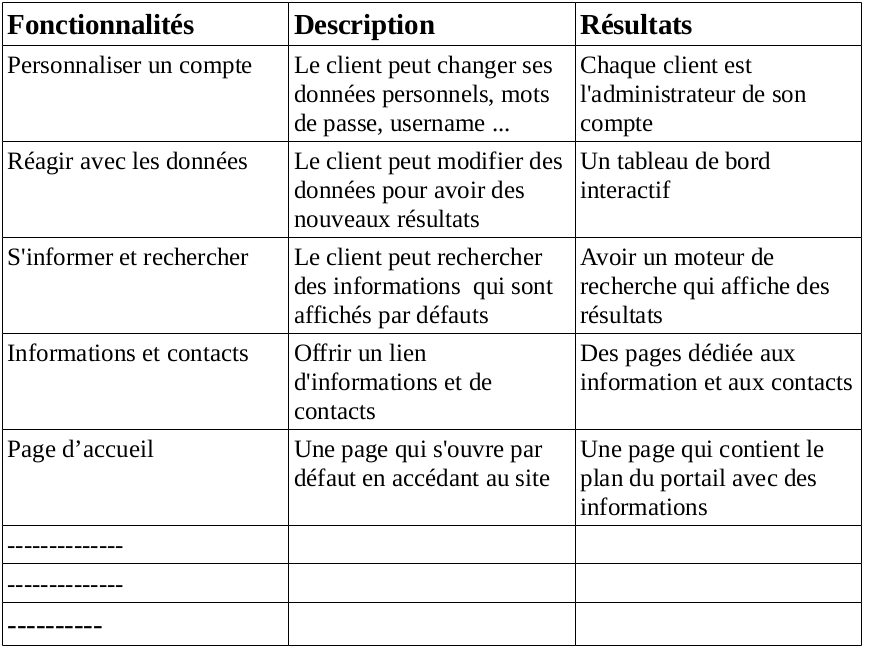
\includegraphics[width=200,height=250]{cdc.png}}
\end{center}
 \\ \\

L'étape suivante de ce stage était l'analyse des donnés, la conception générale et la recherche des solutions pour les problèmes évoqués.



\newpage

\section{Analyse et Conception}


\subsection{Modélisation}

\subsection{Bases de Données}

\subsection{Front-end}

\subsection{Banck-end}

\subsection{Outils}

\newpage

\section{Développement et Implémentation}

\subsection{Symfony}

\subsection{Back Office}

\subsection{Front Office}

\subsection{Temps réel}

\subsection{Sécurité}

\newpage

\section{Résultats et Tests}

\subsection{Démonstrations}

\begin{center}

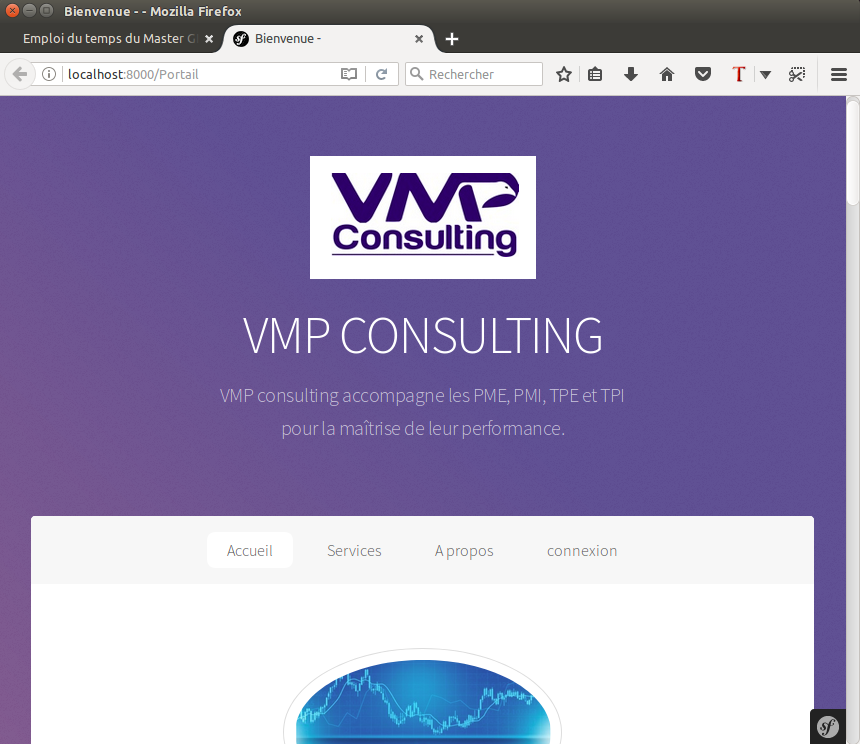
\includegraphics[width=300,height=250]{v1.png}} \\ \\
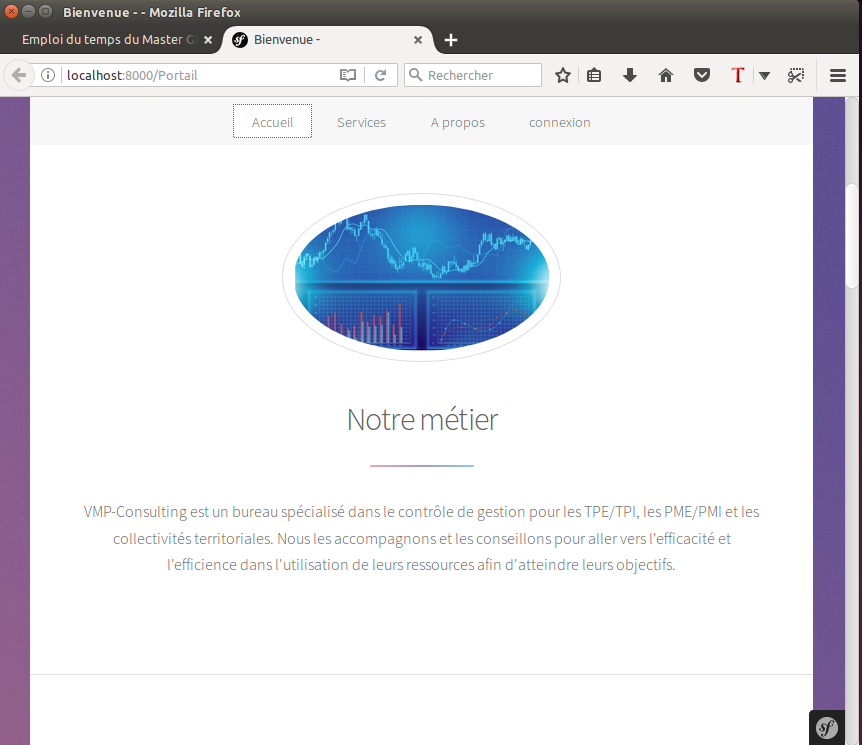
\includegraphics[width=300,height=250]{v2.png}} \\ \\
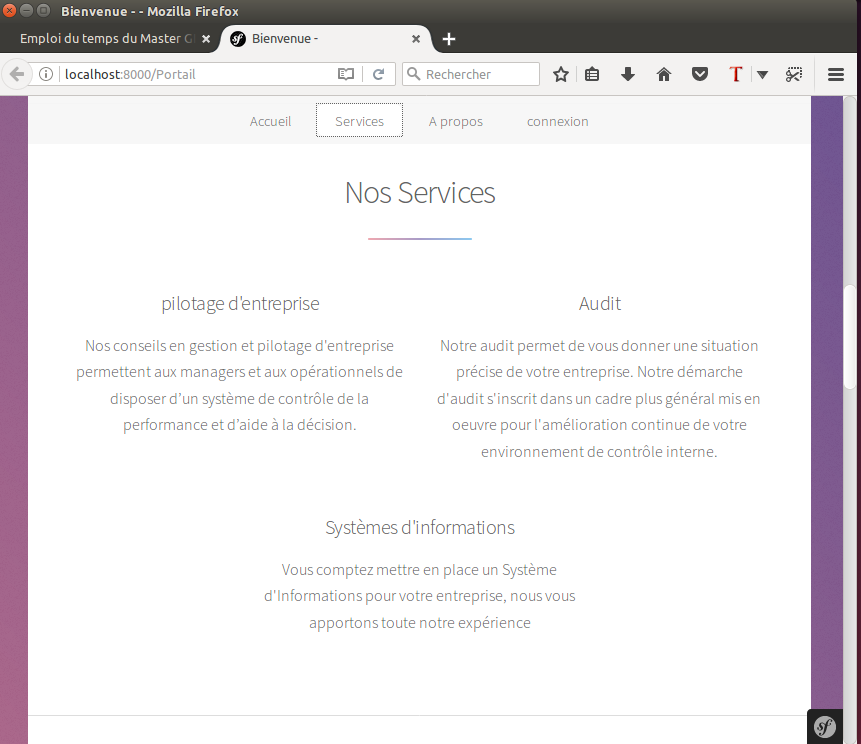
\includegraphics[width=300,height=250]{v3.png}} \\ \\
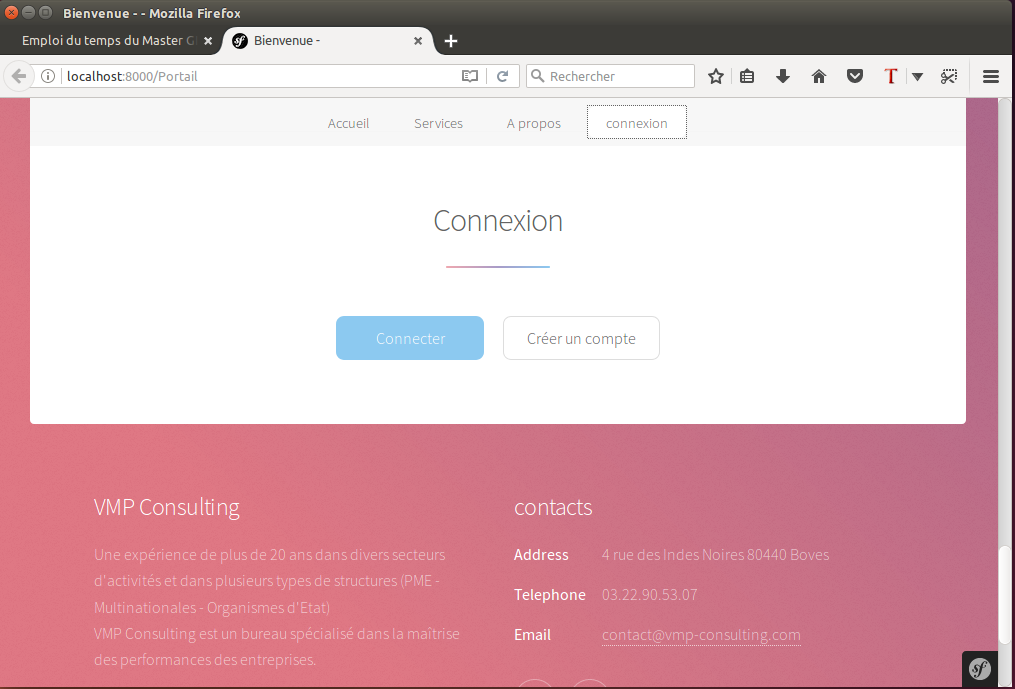
\includegraphics[width=300,height=250]{v4.png}} \\ \\
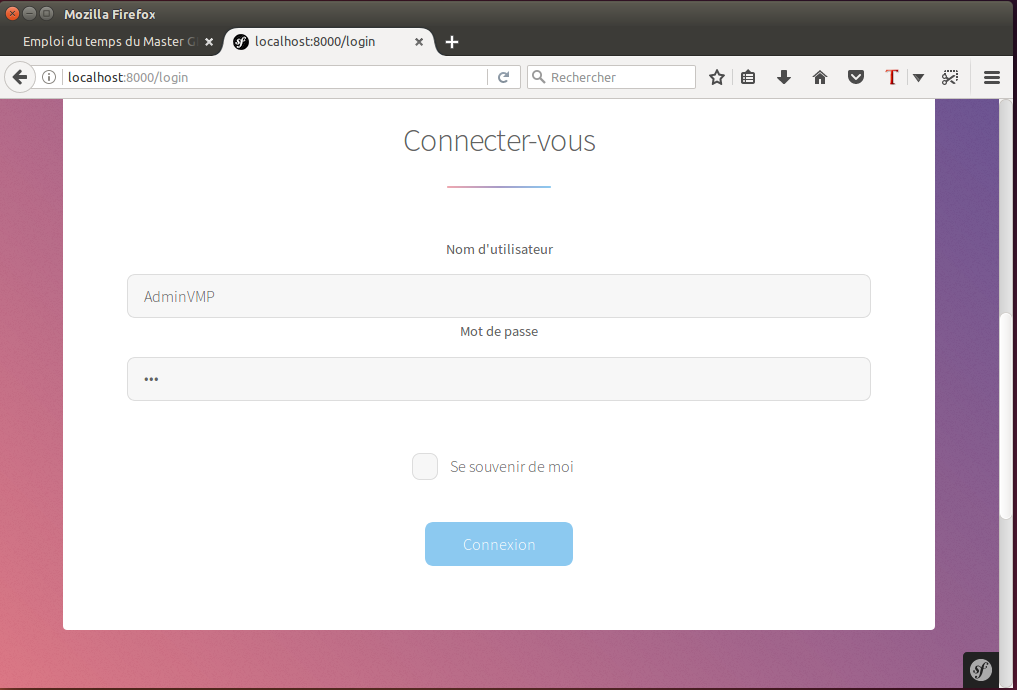
\includegraphics[width=300,height=250]{v5.png}} \\ \\
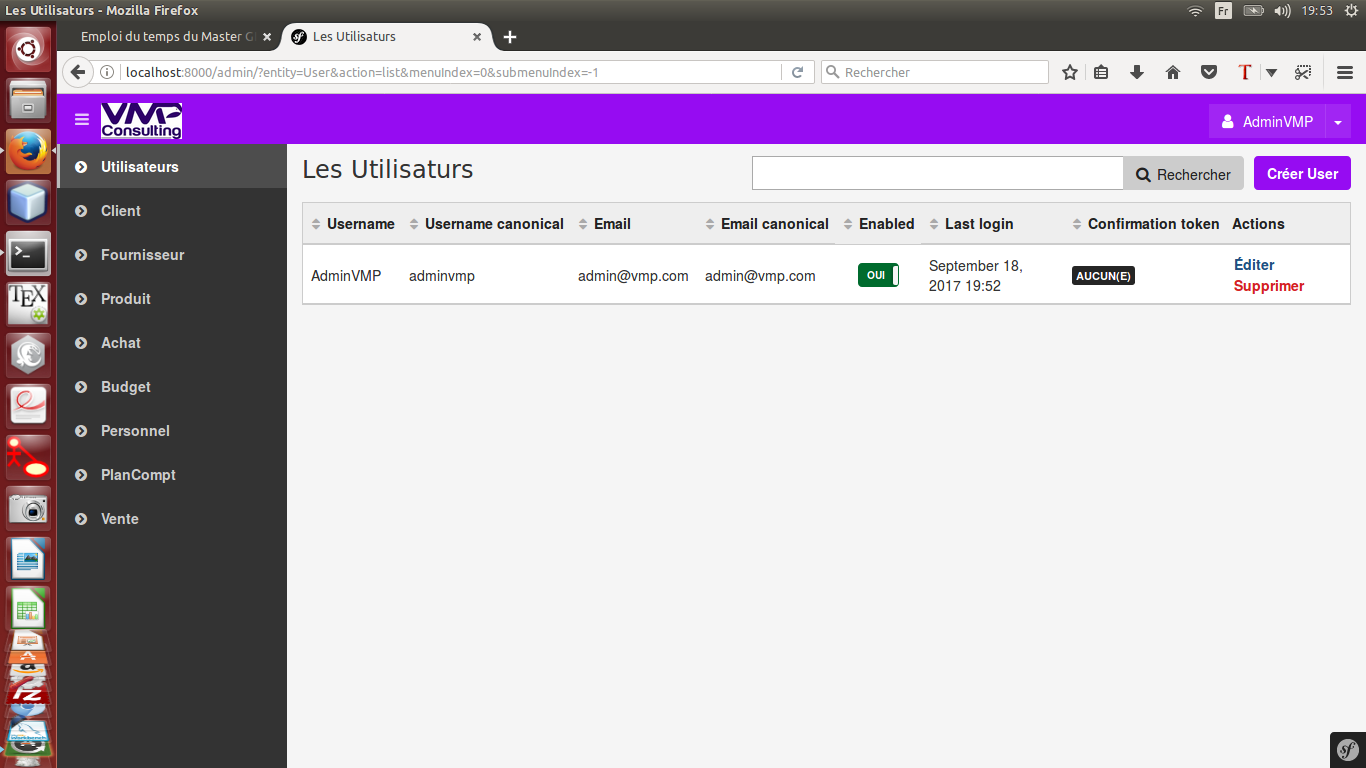
\includegraphics[width=300,height=250]{v6.png}} \\ \\
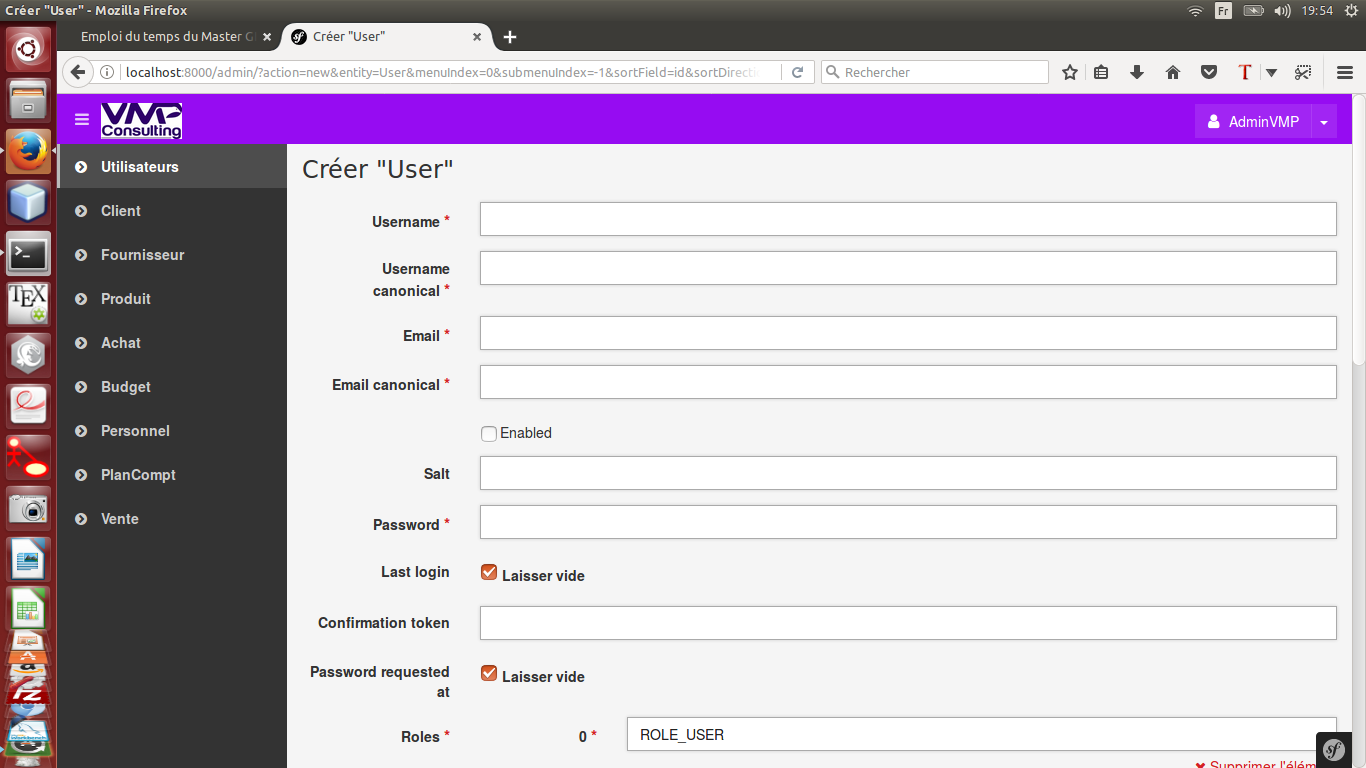
\includegraphics[width=300,height=250]{v7.png}} \\ \\
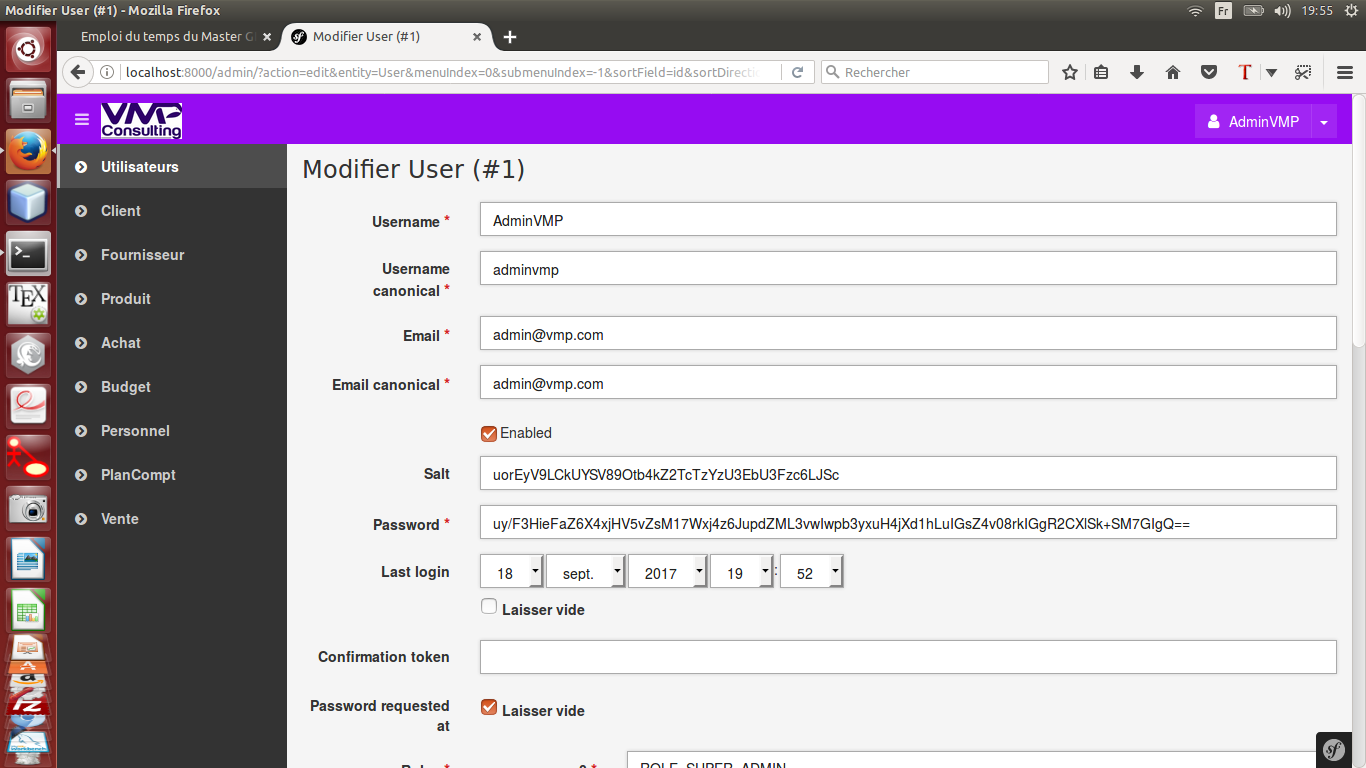
\includegraphics[width=300,height=250]{v8.png}} \\ \\
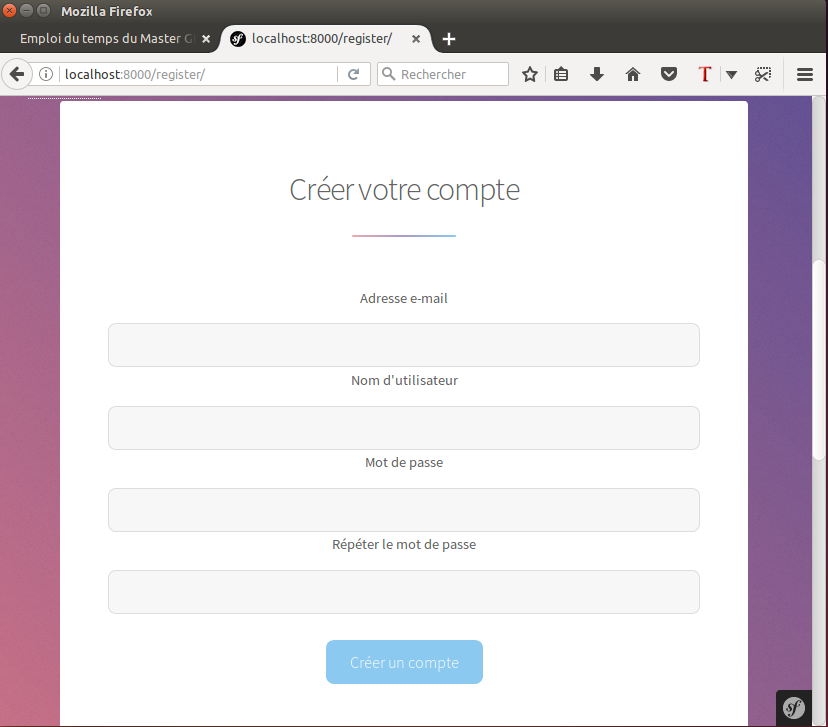
\includegraphics[width=300,height=250]{v9.png}} \\ \\
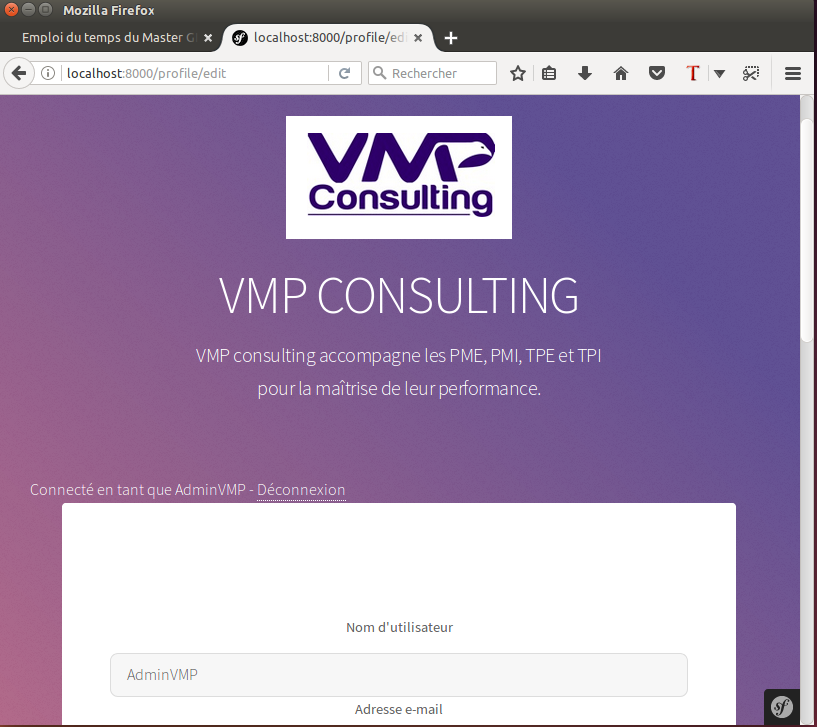
\includegraphics[width=300,height=250]{v10.png}} \\ \\

\end{center}

\subsection{Tests}



\newpage
\section{Conclusion}


\newpage
\section{Bibliographie}


		
\end{document}
